\documentclass[
  bibliography=totoc,     % Literatur im Inhaltsverzeichnis
  captions=tableheading,  % Tabellenüberschriften
  titlepage=firstiscover, % Titelseite ist Deckblatt
]{scrartcl}

%irgendetwas mit Tabelen und Figuren anders Nummerieren 
\usepackage{chngcntr}
\usepackage{longtable} 

\usepackage{titling}

%Textdatein einfügen
\usepackage{verbatim}

% Paket float verbessern
\usepackage{scrhack}

% Warnung, falls nochmal kompiliert werden muss
\usepackage[aux]{rerunfilecheck}

% unverzichtbare Mathe-Befehle
\usepackage{amsmath}
% viele Mathe-Symbole
\usepackage{amssymb}
% Erweiterungen für amsmath
\usepackage{mathtools}

% Fonteinstellungen
\usepackage{fontspec}
% Latin Modern Fonts werden automatisch geladen
% Alternativ zum Beispiel:
%\setromanfont{Libertinus Serif}
%\setsansfont{Libertinus Sans}
%\setmonofont{Libertinus Mono}

% Wenn man andere Schriftarten gesetzt hat,
% sollte man das Seiten-Layout neu berechnen lassen
\recalctypearea{}

% deutsche Spracheinstellungen
\usepackage[ngerman]{babel}


\usepackage[
  math-style=ISO,    % ┐
  bold-style=ISO,    % │
  sans-style=italic, % │ ISO-Standard folgen
  nabla=upright,     % │
  partial=upright,   % ┘
  warnings-off={           % ┐
    mathtools-colon,       % │ unnötige Warnungen ausschalten
    mathtools-overbracket, % │
  },                       % ┘
]{unicode-math}

% traditionelle Fonts für Mathematik
\setmathfont{Latin Modern Math}
% Alternativ zum Beispiel:
%\setmathfont{Libertinus Math}

\setmathfont{XITS Math}[range={scr, bfscr}]
\setmathfont{XITS Math}[range={cal, bfcal}, StylisticSet=1]

% Zahlen und Einheiten
\usepackage[
  locale=DE,                   % deutsche Einstellungen
  separate-uncertainty=true,   % immer Unsicherheit mit \pm
  per-mode=symbol-or-fraction, % / in inline math, fraction in display math
]{siunitx}

\DeclareSIUnit{\channel}{Channel}
\DeclareSIUnit{\year}{a}

% chemische Formeln
\usepackage[
  version=4,
  math-greek=default, % ┐ mit unicode-math zusammenarbeiten
  text-greek=default, % ┘
]{mhchem}

% richtige Anführungszeichen
\usepackage[autostyle]{csquotes}

% schöne Brüche im Text
\usepackage{xfrac}

% Standardplatzierung für Floats einstellen
\usepackage{float}
\floatplacement{figure}{htbp}
\floatplacement{table}{htbp}

% Floats innerhalb einer Section halten
\usepackage[
  section, % Floats innerhalb der Section halten
  below,   % unterhalb der Section aber auf der selben Seite ist ok
]{placeins}

% Seite drehen für breite Tabellen: landscape Umgebung
\usepackage{pdflscape}

% Captions schöner machen.
\usepackage[
  labelfont=bf,        % Tabelle x: Abbildung y: ist jetzt fett
  font=small,          % Schrift etwas kleiner als Dokument
  width=0.9\textwidth, % maximale Breite einer Caption schmaler
]{caption}
% subfigure, subtable, subref
\usepackage{subcaption}

% Grafiken können eingebunden werden
\usepackage{graphicx}
\usepackage{wrapfig}

% schöne Tabellen
\usepackage{booktabs}
\usepackage[table]{xcolor}

% Verbesserungen am Schriftbild
\usepackage{microtype}

% Literaturverzeichnis
\usepackage[
  backend=biber,
  sorting=none
]{biblatex}
% Quellendatenbank
\addbibresource{lit.bib}
\addbibresource{programme.bib}

% Hyperlinks im Dokument
\usepackage[
  german,
  unicode,        % Unicode in PDF-Attributen erlauben
  pdfusetitle,    % Titel, Autoren und Datum als PDF-Attribute
  pdfcreator={},  % ┐ PDF-Attribute säubern
  pdfproducer={}, % ┘
]{hyperref}
% erweiterte Bookmarks im PDF
\usepackage{bookmark}

% Trennung von Wörtern mit Strichen
\usepackage[shortcuts]{extdash}

%\setcounter{tocdepth}{3} % + subsubsections



\author{%
  Benedikt Lütke Lanfer \\%
  \href{mailto:benedikt.luetkelanfer@tu-dortmund.de}{benedikt.luetkelanfer@tu-dortmund.de}%
  \and%
  Enno Wellmann \\%
  \href{mailto:enno.wellmann@tu-dortmund.de}{enno.wellmann@tu-dortmund.de}%
}
\publishers{TU Dortmund – Fakultät Physik}


\newcommand*\diff{\mathop{}\!\mathrm{d}}

\NewDocumentCommand \OverfullCenter {+m} {
\noindent\makebox[\linewidth]{#1} }

\usepackage{adjustbox}


% %Tabellen und Figuren Einstellung
% \counterwithout{table}{section}
% \counterwithout{figure}{section}
% \renewcommand{\thetable}{\Roman{table}}
% \renewcommand{\thefigure}{\Roman{figure}}

%Richtiges Einrücken
\setlength{\parindent}{0pt}


\title{V60:\\ Der Diodenlaser}
\author{Benedikt Lütke Lanfer \and Enno Wellmann}
\date{15. April 2024}
\publishers{TU Dortmund – Fakultät Physik}
\graphicspath{./Materialien}

\begin{document}
\begin{titlingpage}
    \begin{center}
        \begin{Huge}
            \textbf{\thetitle\\}
        \end{Huge}
    \end{center}
    \vspace{4cm}
    
\includegraphics[width=\textwidth]{Bilder/Logo_TU.png} \\
    \vspace{4cm}
    \begin{center}
        \begin{huge}
            \theauthor\\
        \end{huge}
        \vspace{0.5cm}
        \begin{Large}
            benedikt.luetkelanfer@tu-dortmund.de\\
            enno.wellmann@tu-dortmund.de\\
            \vspace{1.4cm}
            Bearbeitet: \today\\
            Durchgeführt: \thedate\\
            TU Dortmund – Fakultät Physik\\
        \end{Large}
    \end{center}
\end{titlingpage}
\tableofcontents
\newpage

\section{Zielsetzung}
Ziel dieses Versuches ist ein Diodenlaser richtig zu kalibrieren, sodass damit das Absorption Spectrum von Rubidium vermessen werden kann. 
%---------------------------------------------------------------------------------------------------------------------------------------------------------------%

\section{Theorie}
Bevor der Erfindung des Diodenlasers waren die herkömmlichen Farblaser komplex und teuer. 
Außerdem waren sie schwierig zu bedienen, welches sich durch die Entwicklung der Verstellbaren Halbleiter Diodenlasers, mit enger Bandbreite, stark verbesserte. 

\subsection{Funktionsweise eines Diodenlasers}
Das prinzipielle Funktionsprinzip eines Diodenlasers unterscheidet sich am Anfang nicht von einer Halbleiterdiode. 
Bei dieser werden zwei Halbleiter mit n und p Dotierung aneinander gebracht, wodurch eine Grenzschicht oder auch Aktivschicht entsteht.  
Wenn nun ein Strom durch diese Grenzschicht fließt entstehen Elektronen Lochpaare, welche in dieser Aktienschicht sich wieder auslöschen. 
Bei diesem Prozess geben die Elektronen Licht mit der Wellenlänge ihrer Energie ab. 
Die Energie hängt wiederum fest von der Bandstruktur des Halbleiters ab.

\begin{wrapfigure}{r}{0.5\textwidth}
    \centering
    \vspace{-20pt}
    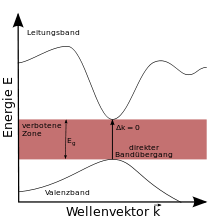
\includegraphics[width=0.4\textwidth]{Bilder/Bandstruktur.png} 
    \caption{Bsp: optischer Übergang in einer Bandstruktur \cite{Bandstruktur}}
    \label{fig:Bandstruktur}
\end{wrapfigure}

In der nebenstehenden Abbildung \eqref{fig:Bandstruktur} ist eine vereinfachte Bandstruktur beispielhaft abgebildet. 
Wenn nun Elektronen-Lochpaare sich gegenseitig eliminieren, so findet ein optischer Übergang vom Leitungsband ins Valenzband statt. 
Dieser hat eine feste Energie und somit hat auch das emittierte Licht eine nahezu feste Wellenlänge, 
welche in einem dünnen Channel im Chip \eqref{fig:Schemata} eingeschränkt ist. 
Die Enden dieses Chips verhalten sich, durch ihren hohen Brechungsindex, wie partiell reflektierende Spiegel, die das Licht teils einschließen. 
Wenn das Licht im Chip hin und her reflektiert wird, regt es angeregte Atome ab, welche wiederum Licht mit der exakt selben Wellenlänge und Richtung emittiert. 
Dieses wird stimulierte Emissionen genannt, welche dafür sorgen, dass Licht einer bestimmten Wellenlänge verstärkt wird.  

\begin{figure}[H]
    \centering
    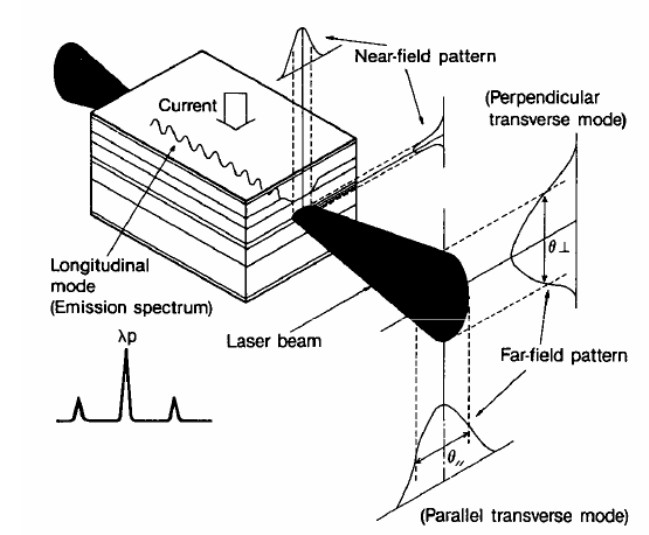
\includegraphics[width=\textwidth]{Bilder/Schemata.png} 
    \caption{Aufbau des Diodenchips \cite{man:v60}}
    \label{fig:Schemata}
\end{figure}

Das Licht, welches dann aus dem Chip austritt, ist aufgrund der schmalen Austrittsfläche stark elliptisch und divergent, welches mit einer Linse korrigiert wird. 
Danach kommt ein Beugungsgitter, welches je nach Winkel eine bestimmte Wellenlänge des Lichtes wieder in den Laser zurückwirft. 
Dadurch wird im Laser die stimulierte Emission vermehrt mit dieser Wellenlänge durchgeführt und der LASER strahlt weniger anders welliges Licht aus.
Damit kann man den LASER genauer auf die gewünschte Wellenlänge einstellen, die gebraucht wird. 
Die genaue Feineinstellung des LASER wird im folgenden Abschnitt erklärt. 

\newpage
\subsection{Beiträge zur Gesamtintensität}
Die verschiedenen Anteile an der Gesamtintensität des LASER sind in folgender Abbildung abgebildet. 

\begin{figure}[H]
    \centering
    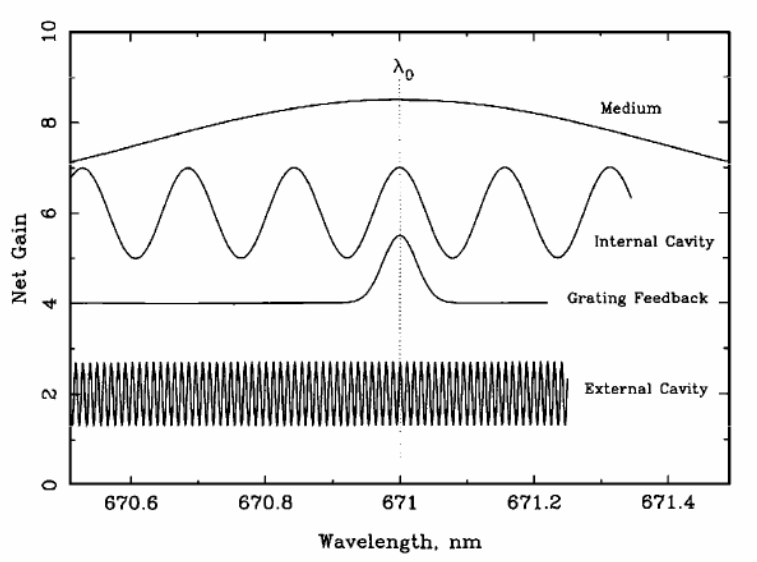
\includegraphics[width=0.9\textwidth]{Bilder/LASER_Moden.png} 
    \caption{Die verschiedenen Beiträge zur Gesamtintensität \cite{man:v60}}
    \label{fig:Moden}
\end{figure}

\begin{description}
    \item[1.Das Medium] des Halbleiterchips und dessen Bandlücke ist stark Temperatur abhängig. 
    Dadurch wird bei höheren Temperaturen die Wellenlänge größer ($\qty{0.23}{\nano\meter\per\celsius}$). 
    \item[2.Die innerer Cavity] oder auch optischer Hohlraumresonator sorgt für das sich ganzzahlige vielfache der Wellenlänge bilden, die stehende Wellen im Chip erzeugen. 
    Die Periodizität dessen nennt man "freier Spektralbereich" und beträgt für diesen LASER $\Delta_{FSR} \approx  \qty{60}{\giga\hertz}$. 
    Auch hier ist die Wellenlänge Temperatur empfindlich aber hängt auch vom Strom ab. 
    Dieser kann sowohl die Temperatur wieder erhöhen als auch die Elektronen-Lochpaar-Konzentration ändern. 
    \item[3.Das Beugungsgitter Feedback] sorgt für besseres regulieren der gewünschten Wellenlänge mit stimulierte Emissionen. 
    Durch Ändern des Winkels $\theta $ des Gitters wird die richtig Wellenlänge, nach $\lambda =2d \sin\theta $ in den LASER zurückgeworfen. 
    \item[4.Die äußerer Cavity] ist deutlich größer als die innere mit $\Delta_{FSR} \approx  \qty{10}{\giga\hertz}$ und kann durch piezo-electric tranducer verändert werden. 
\end{description}

\subsection{Mode Hop}
Die verschiedenen Einstellungsmöglichkeiten beim LASER reagieren nicht alle gleich schnell oder linear auf Veränderungen.
Wenn die innere Cavity konstant gehalten wird und nur der Winkel des Gitters und die äußere Cavity verändert werden kann ein Mode Hop auftreten \eqref{fig:Hop}.
Am Anfang seien die Intensitätsmaxima von inneren (Int0) und äußere Cavity sowie des Gitterfeedbacks(e0) überlagert. Falls nun Veränderungen vorgenommen werden, 
bleibt das innere Maximum bei derselben Wellenlänge, während das andere Maxima sich verschiebt. 
Der LASER bleibt jedoch bei der bisherigen betriebenen Wellenlänge. 
Erst, wenn das Maximum von äußere Cavity und das des Gitters sich weit genug verschoben haben, gibt es ein großen Mode Hop, 
da das zweite Maximum (Int1) der inneren Cavity mehr überlagert als das erste (Int0).
Dadurch macht die Frequenz des LASER ein $\qty{20}{\giga\hertz}$ Sprung. 

\begin{figure}[H]
    \centering
    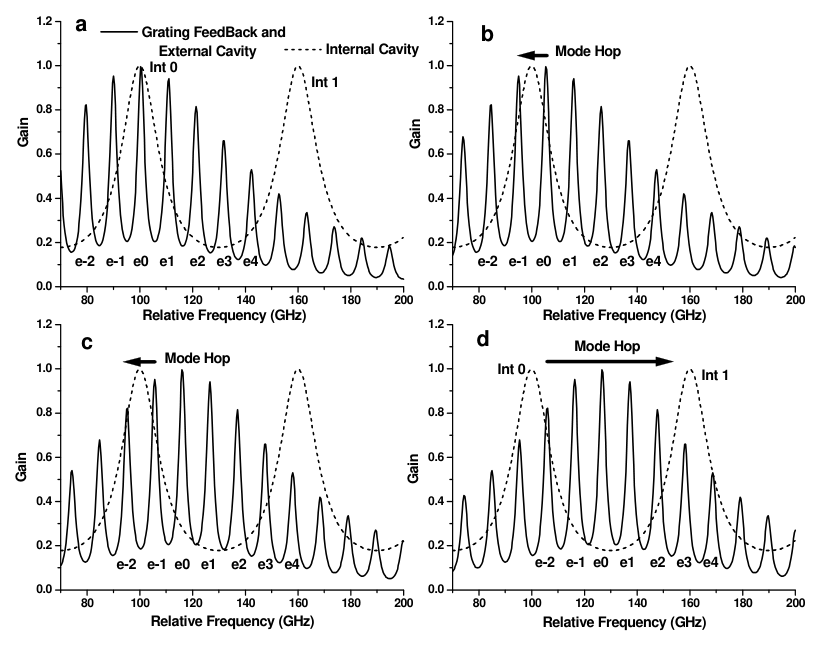
\includegraphics[width=\textwidth]{Bilder/Mode_Hop.png} 
    \caption{Grafische Darstellung eines Mode Hops \cite{man:v60}}
    \label{fig:Hop}
\end{figure}

Um die LASER ohne diese Mode Hop genauer einstellen zu können muss auch die innere Cavity, durch Veränderung des Stroms, gleichzeitig angepasst werden.
Dadurch kann man die gesamte Frequenzbreite des LASER abdecken und kalibrieren. 


% \subsection{Fehlerrechnung}
% Für die Fehlerrechnung werden alle \textbf{Mittelwerte} von $N$ Messungen folgendermaßen berechnet:

% \begin{equation}
%     \overline{x} = \frac{1}{N} \cdot \sum_{i=1}^N x_i
%     \label{eqn:Mittelwert}
% \end{equation}

% und alle \textbf{Standardabweichungen zum Mittelwert} mit:

% \begin{equation}
%     \increment\overline{x} = \sqrt{\frac{1}{N\cdot(N-1)}\cdot\sum_{i=1}^N (x_i-\overline{x})^2}
%     \label{eqn:St_Mittelwert}
% \end{equation}

% Der Fehler für zusammenhängende Messwerte wird dann mit der \textbf{Gaußschen Fehlerfortpflanzung} berechnet:

% \begin{equation}
%     \increment{f} = \sqrt{ \sum_{i = 1}^{N}  \biggl(\frac{\partial{f}}{\partial{x_i}}\biggr)^2\cdot(\increment{x_i})^2}
%     \label{eqn:Gauss}
% \end{equation}

% Die Fehlerfortpflanzung wird mit Uncertainties in Python \cite{uncertainties} ermittelt.

%---------------------------------------------------------------------------------------------------------------------------------------------------------------%

\section{Durchführung}


%---------------------------------------------------------------------------------------------------------------------------------------------------------------%

\section{Auswertung}

\subsection{Schwellwert für die LASER Bildung}
In Abbildung \ref{fig:laser_karte} ist zu sehen wie der Laser auf die Karte strahlt.
Das für Menschen unsichtbare Licht mit einer Wellenlänge von 780 nm kann mit der Kamera eingefangen werden. %Vielleicht nicht ganz der richtige Ort für diese Anmerkung
Bei einem Strom unterhalb eines Schwellwerts ist ein schwacher Punkt auf der Karte zu erkennen.
Oberhalb davon leuchtet dieser Punkt erheblich stärker und bildet kleine Leuchtflecken Rund um den Leuchtpunkt.
Der Wert wird ermittelt indem sich schrittweise von beiden Seiten daran angenähert wird.
\begin{tabular}[table-format=2.1]{S S}
    \toprule
    {Unter dem Schwellwert} & {Über dem Schwellwert} \\
    {$I/\si{\milli\ampere}$} & {$I/\si{\milli\ampere}$}\\
    \midrule
    34.8  & 36.0 \\
    34.6  & 34.9 \\
          & 34.8 \\
    \bottomrule    
\end{tabular}
Es ergibt sich ein Schwellwert bei $I = \qty{34.8}{\milli\ampere}$.

\begin{figure}
    \centering
    \subfloat[Lichtpunkt im dioden Zustand des Lasers]{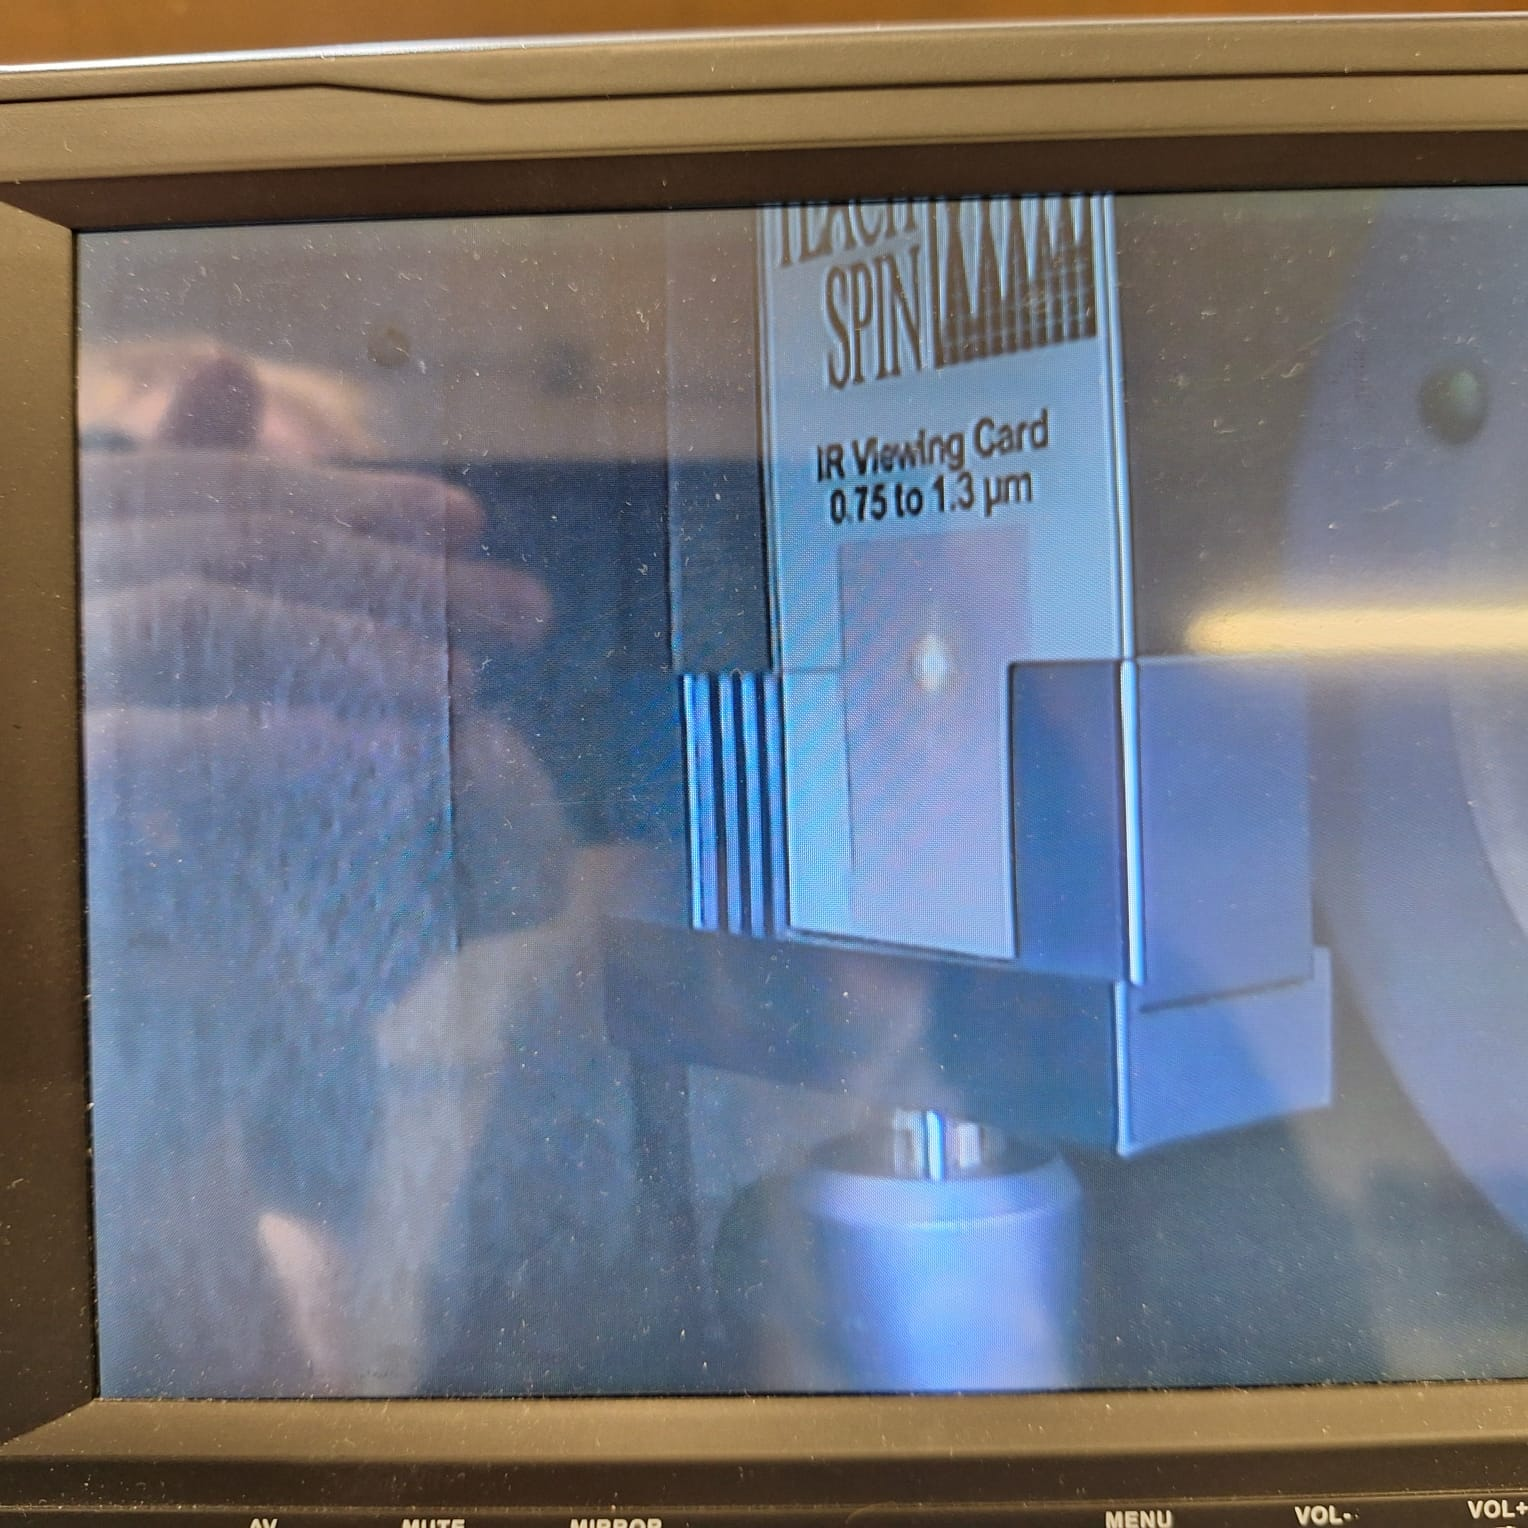
\includegraphics[width=0.4\textwidth]{./Materialien/karte_laser_schwach.jpeg}}
    \hfill
    \subfloat[Licht im Laser Zustand]{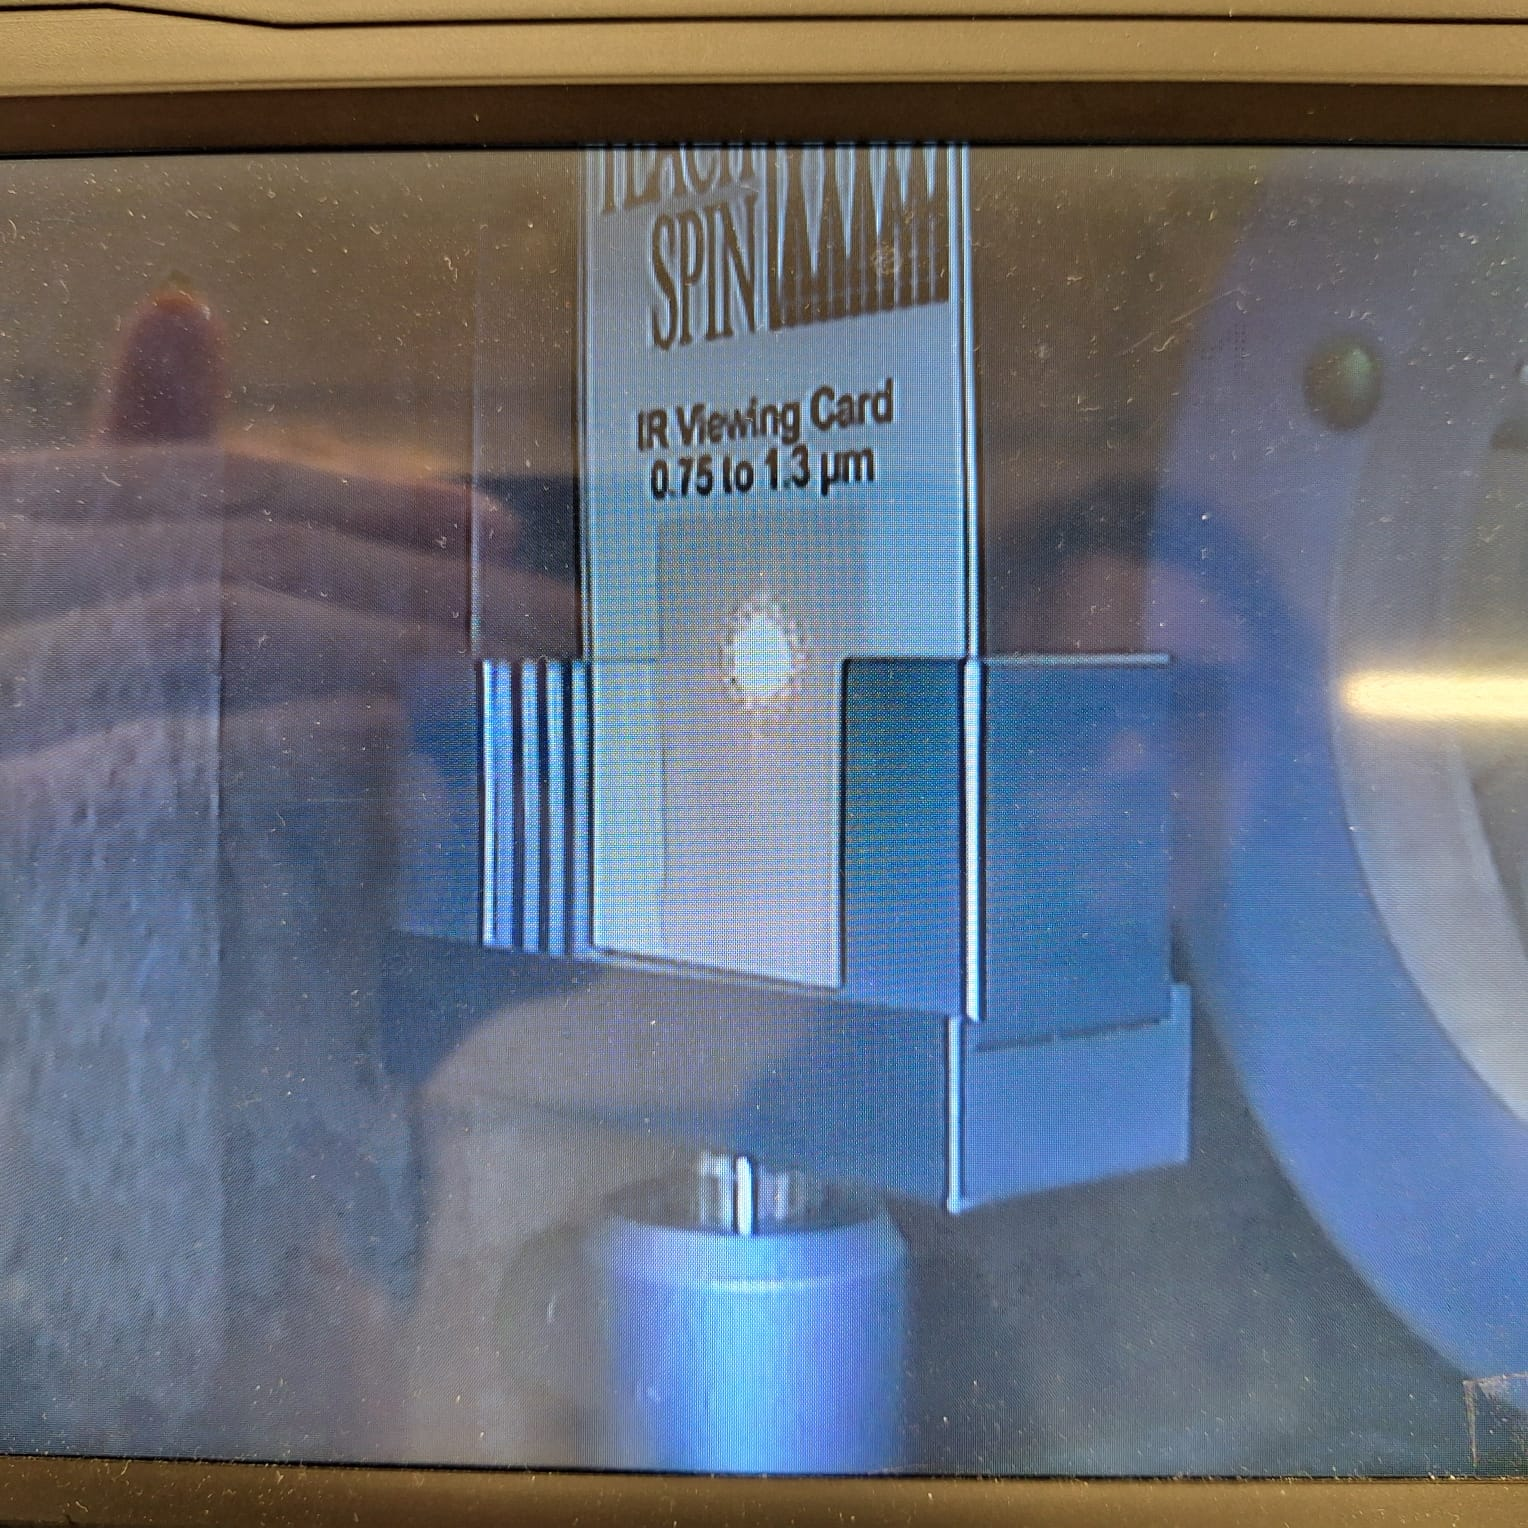
\includegraphics[width=0.4\textwidth]{./Materialien/karte_laser_stark.jpeg}}
    \caption{Zustände des Lasers}\label{fig:laser_karte}
\end{figure}

\subsection{Rubidium Fluoreszenz}
Bei einer Temperatur des Rb Gases von 50 °C kann mit der Kamera die Fluoreszenz beobachtet werden.
In Abbildung \ref{fig:rb_fluoreszenz} ist das Leuchten des Gases zu erkennen.
Entlang des Laserstrahls leuchtet das Gas verstärkt.
\begin{figure}
    \centering
    \subfloat[ohne Fluoreszenz]{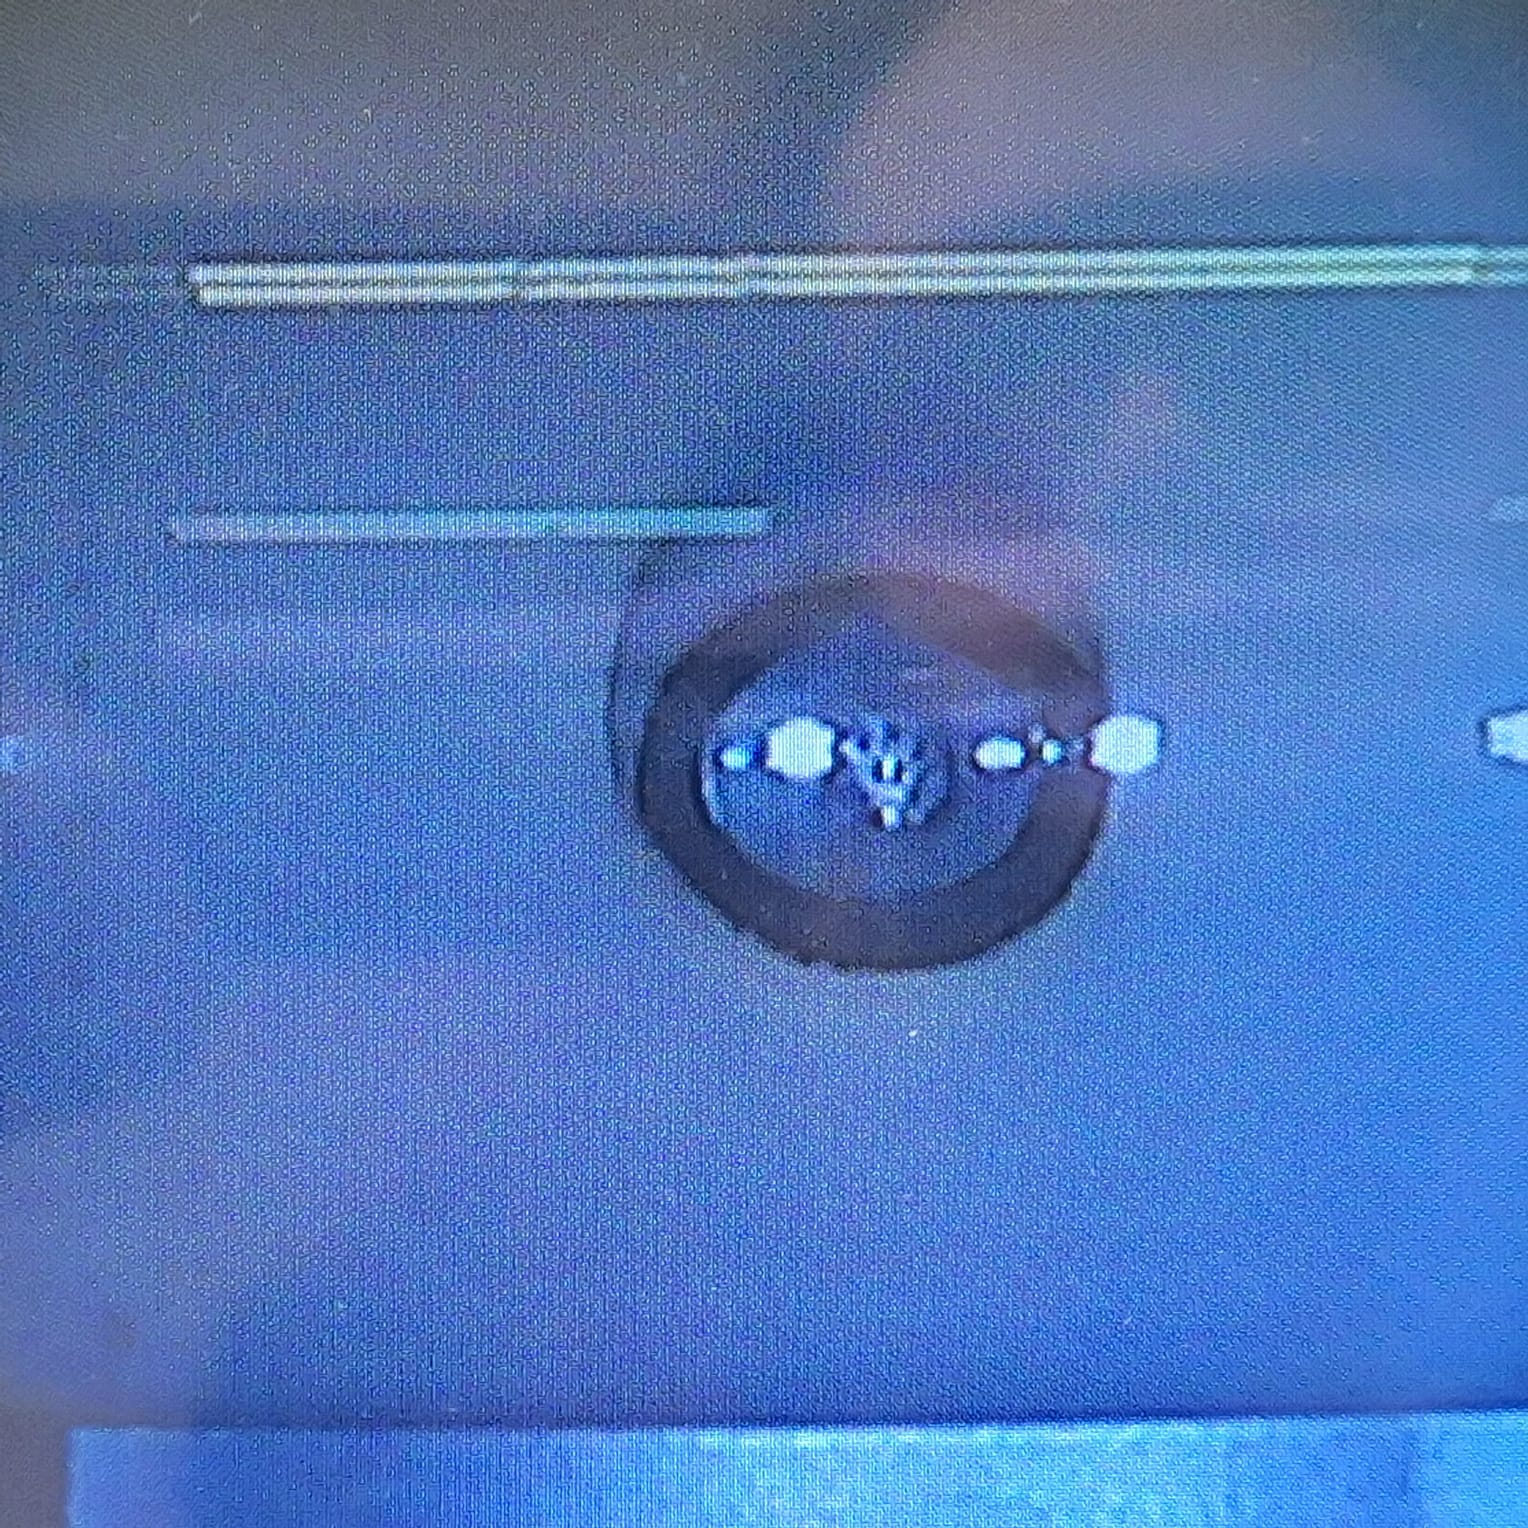
\includegraphics[width=0.4\textwidth]{./Materialien/Rb_Zelle_keine_Floureszenz.jpeg}}
    \hfill
    \subfloat[mit Fluoreszenz]{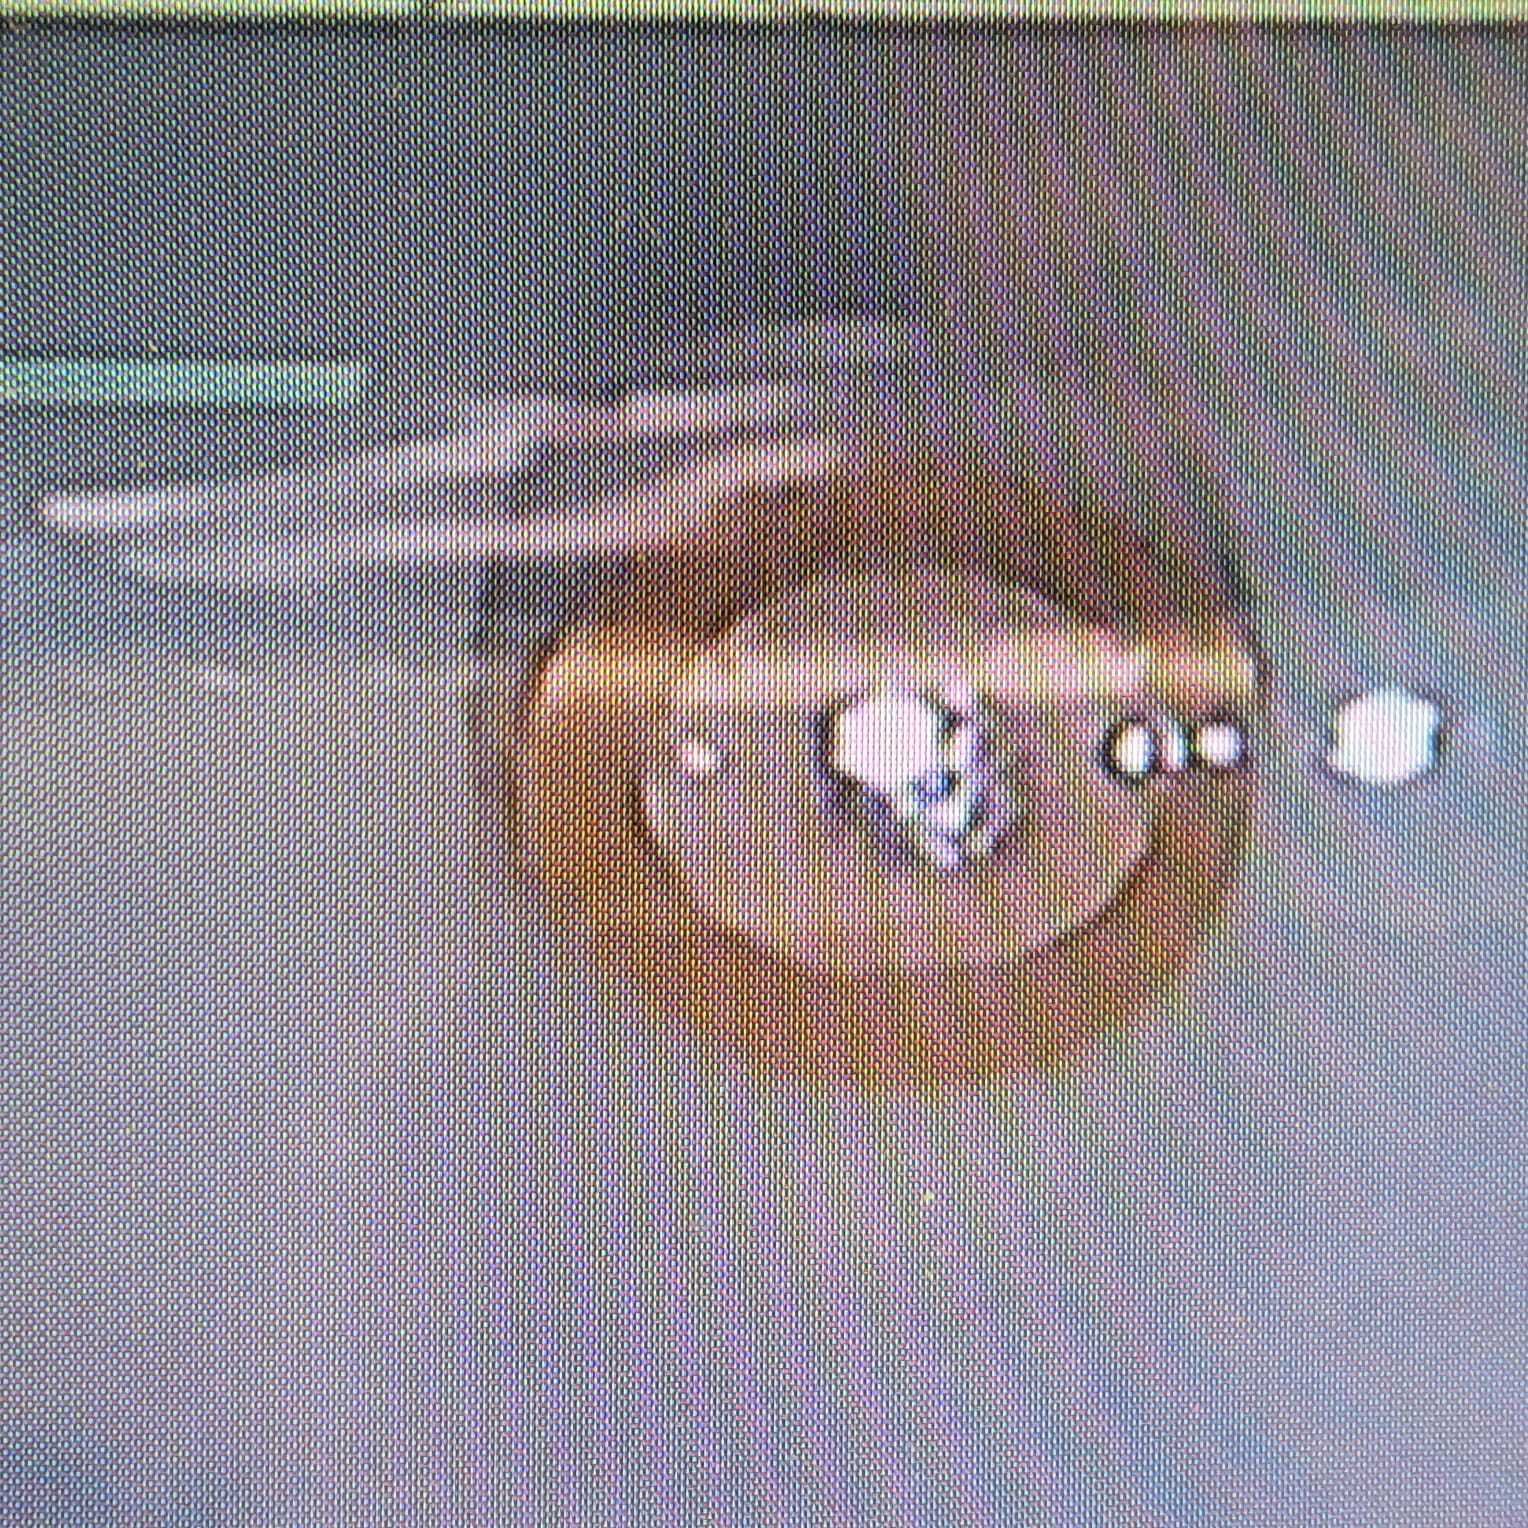
\includegraphics[width=0.4\textwidth]{./Materialien/Rb_Zelle_Floureszenz.jpeg}}
    \caption{Rb Zelle mit und ohne sichtbarer Fluoreszenz.}\label{fig:rb_fluoreszenz}
\end{figure}

\subsection{Absorptionsspektrum}
Durch Manipulieren des DC-Offsets und durch manipulieren des Diffraction gratings
lässt sich das Spektrum in einer kontinuierlichen Art und Weise darstellen. % mehr als nur der DC offset
Der Abgleich zwischen Referenzsignal und gemessenen Signal ergibt ein Absorptionsspektrum mit ebener Grundlinie.
Das entstehende Spektrum ist in Abbildung \ref{fig:spektrum} zu sehen.

\begin{figure}
    \centering
    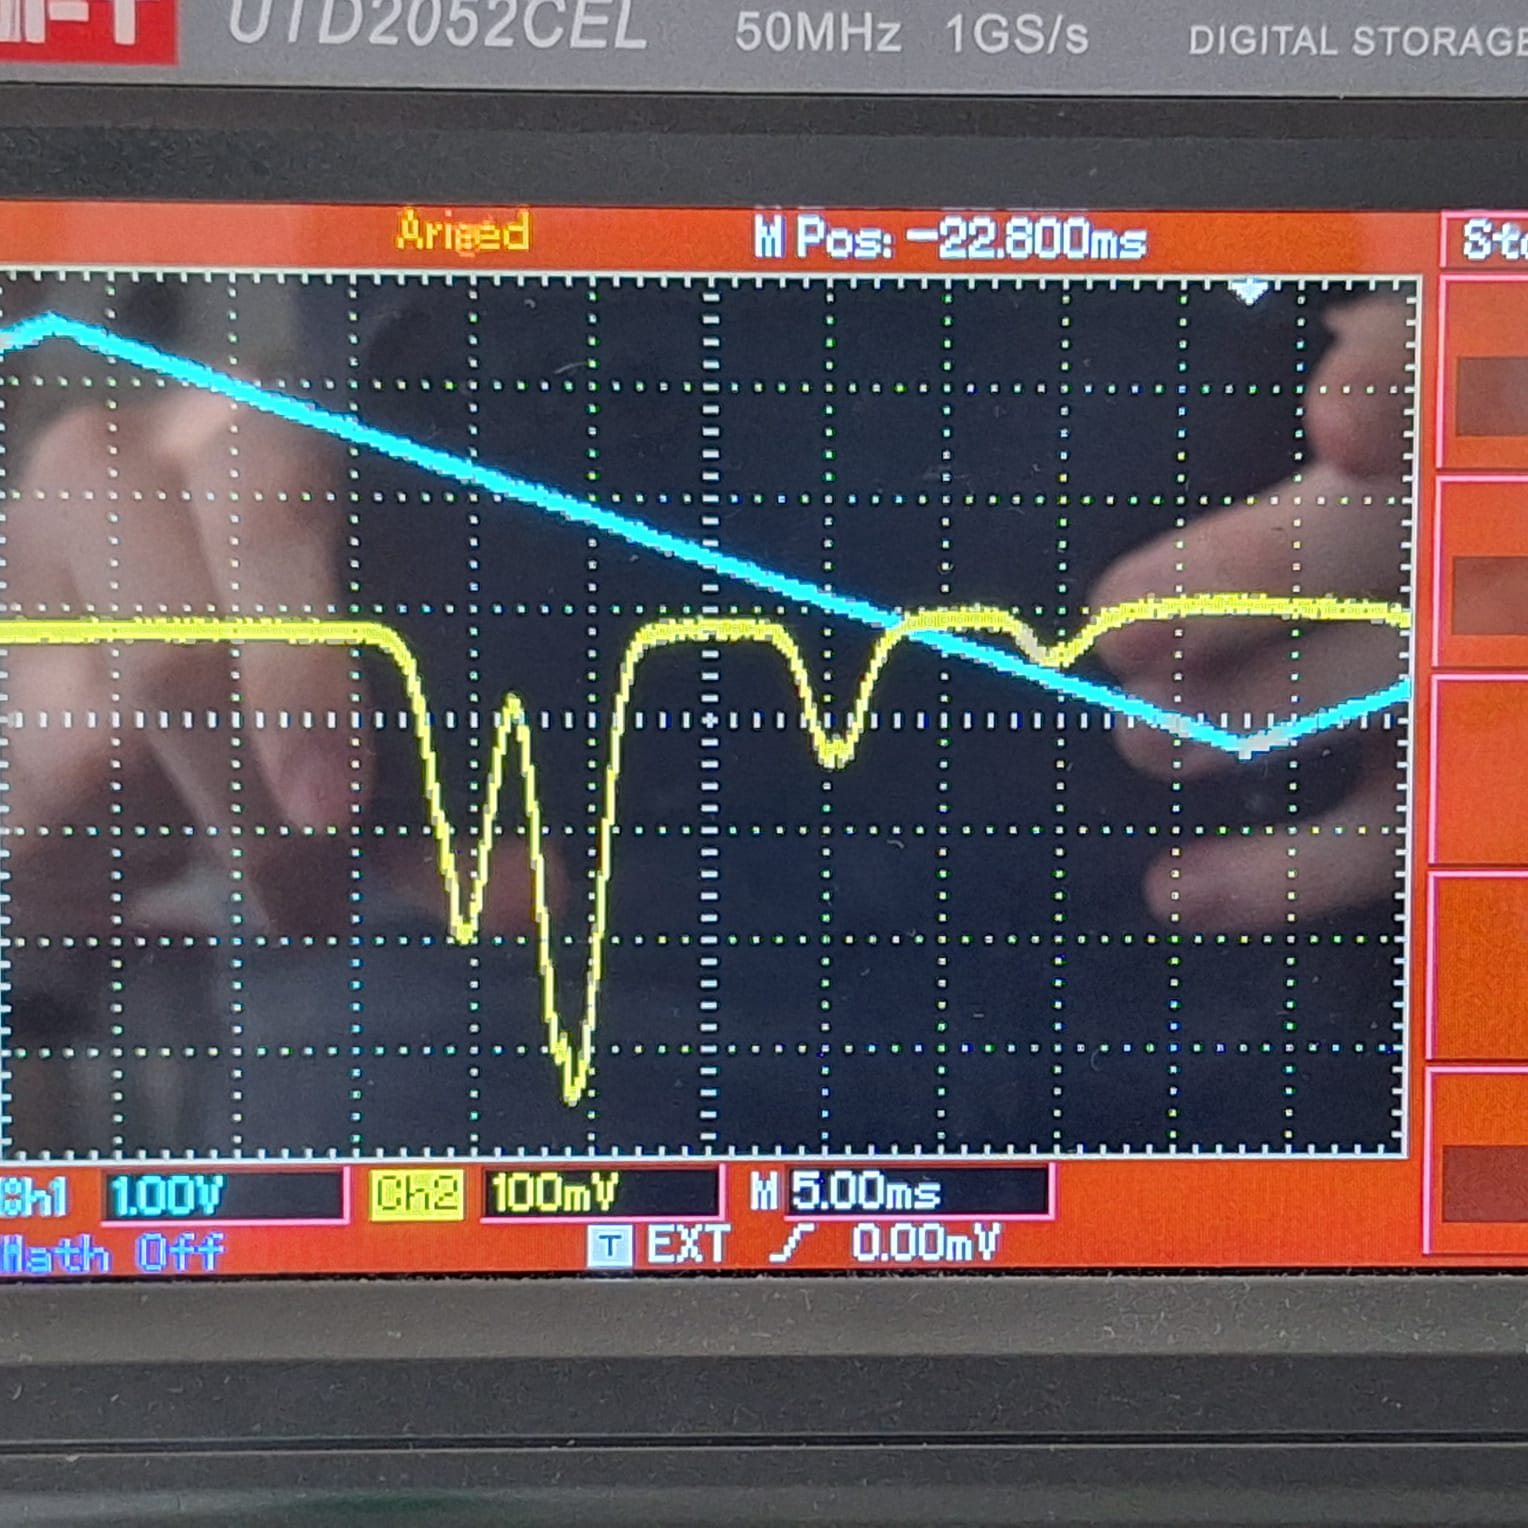
\includegraphics[width=0.4\textwidth]{./Materialien/spektrum.jpeg}
	\caption{Ausgeglichenes Absorptionsspektrum}\label{fig:spektrum}
\end{figure}

%---------------------------------------------------------------------------------------------------------------------------------------------------------------%

\section{Diskussion}
Der Diodenlaser wurde in diesem Experiment erfolgreich in Betrieb genommen.
Durch die Verwendung der Kamera und der sichtbar machenden Karte konnte der Weg des Laserstrahls nachvollzogen werden.
In der mit Rubidiumgas gefüllten Kammer konnte Fluoreszenz beobachtet werden und das Absorptionsspektrum in Abhängigkeit
der Wellenlänge gemessen werden.
Das durchgeführte Experiment ist eine funktionierende Grundlage von der ausgehend
 eine weitergehende Spektralanalyse durchgeführt werden könnte. 


%---------------------------------------------------------------------------------------------------------------------------------------------------------------%

\printbibliography

\end{document}
